\PassOptionsToPackage{unicode=true}{hyperref} % options for packages loaded elsewhere
\PassOptionsToPackage{hyphens}{url}
%
\documentclass[12pt,]{article}
\usepackage{lmodern}
\usepackage{amssymb,amsmath}
\usepackage{ifxetex,ifluatex}
\usepackage{fixltx2e} % provides \textsubscript
\ifnum 0\ifxetex 1\fi\ifluatex 1\fi=0 % if pdftex
  \usepackage[T1]{fontenc}
  \usepackage[utf8]{inputenc}
  \usepackage{textcomp} % provides euro and other symbols
\else % if luatex or xelatex
  \usepackage{unicode-math}
  \defaultfontfeatures{Ligatures=TeX,Scale=MatchLowercase}
\fi
% use upquote if available, for straight quotes in verbatim environments
\IfFileExists{upquote.sty}{\usepackage{upquote}}{}
% use microtype if available
\IfFileExists{microtype.sty}{%
\usepackage[]{microtype}
\UseMicrotypeSet[protrusion]{basicmath} % disable protrusion for tt fonts
}{}
\IfFileExists{parskip.sty}{%
\usepackage{parskip}
}{% else
\setlength{\parindent}{0pt}
\setlength{\parskip}{6pt plus 2pt minus 1pt}
}
\usepackage{hyperref}
\hypersetup{
            pdftitle={Introduction to ggplot2},
            pdfauthor={Andy Grogan-Kaylor},
            pdfborder={0 0 0},
            breaklinks=true}
\urlstyle{same}  % don't use monospace font for urls
\usepackage[margin=1.0in]{geometry}
\usepackage{color}
\usepackage{fancyvrb}
\newcommand{\VerbBar}{|}
\newcommand{\VERB}{\Verb[commandchars=\\\{\}]}
\DefineVerbatimEnvironment{Highlighting}{Verbatim}{commandchars=\\\{\}}
% Add ',fontsize=\small' for more characters per line
\newenvironment{Shaded}{}{}
\newcommand{\AlertTok}[1]{\textcolor[rgb]{1.00,0.00,0.00}{#1}}
\newcommand{\AnnotationTok}[1]{\textcolor[rgb]{0.00,0.50,0.00}{#1}}
\newcommand{\AttributeTok}[1]{#1}
\newcommand{\BaseNTok}[1]{#1}
\newcommand{\BuiltInTok}[1]{#1}
\newcommand{\CharTok}[1]{\textcolor[rgb]{0.00,0.50,0.50}{#1}}
\newcommand{\CommentTok}[1]{\textcolor[rgb]{0.00,0.50,0.00}{#1}}
\newcommand{\CommentVarTok}[1]{\textcolor[rgb]{0.00,0.50,0.00}{#1}}
\newcommand{\ConstantTok}[1]{#1}
\newcommand{\ControlFlowTok}[1]{\textcolor[rgb]{0.00,0.00,1.00}{#1}}
\newcommand{\DataTypeTok}[1]{#1}
\newcommand{\DecValTok}[1]{#1}
\newcommand{\DocumentationTok}[1]{\textcolor[rgb]{0.00,0.50,0.00}{#1}}
\newcommand{\ErrorTok}[1]{\textcolor[rgb]{1.00,0.00,0.00}{\textbf{#1}}}
\newcommand{\ExtensionTok}[1]{#1}
\newcommand{\FloatTok}[1]{#1}
\newcommand{\FunctionTok}[1]{#1}
\newcommand{\ImportTok}[1]{#1}
\newcommand{\InformationTok}[1]{\textcolor[rgb]{0.00,0.50,0.00}{#1}}
\newcommand{\KeywordTok}[1]{\textcolor[rgb]{0.00,0.00,1.00}{#1}}
\newcommand{\NormalTok}[1]{#1}
\newcommand{\OperatorTok}[1]{#1}
\newcommand{\OtherTok}[1]{\textcolor[rgb]{1.00,0.25,0.00}{#1}}
\newcommand{\PreprocessorTok}[1]{\textcolor[rgb]{1.00,0.25,0.00}{#1}}
\newcommand{\RegionMarkerTok}[1]{#1}
\newcommand{\SpecialCharTok}[1]{\textcolor[rgb]{0.00,0.50,0.50}{#1}}
\newcommand{\SpecialStringTok}[1]{\textcolor[rgb]{0.00,0.50,0.50}{#1}}
\newcommand{\StringTok}[1]{\textcolor[rgb]{0.00,0.50,0.50}{#1}}
\newcommand{\VariableTok}[1]{#1}
\newcommand{\VerbatimStringTok}[1]{\textcolor[rgb]{0.00,0.50,0.50}{#1}}
\newcommand{\WarningTok}[1]{\textcolor[rgb]{0.00,0.50,0.00}{\textbf{#1}}}
\usepackage{longtable,booktabs}
% Fix footnotes in tables (requires footnote package)
\IfFileExists{footnote.sty}{\usepackage{footnote}\makesavenoteenv{longtable}}{}
\usepackage{graphicx,grffile}
\makeatletter
\def\maxwidth{\ifdim\Gin@nat@width>\linewidth\linewidth\else\Gin@nat@width\fi}
\def\maxheight{\ifdim\Gin@nat@height>\textheight\textheight\else\Gin@nat@height\fi}
\makeatother
% Scale images if necessary, so that they will not overflow the page
% margins by default, and it is still possible to overwrite the defaults
% using explicit options in \includegraphics[width, height, ...]{}
\setkeys{Gin}{width=\maxwidth,height=\maxheight,keepaspectratio}
\setlength{\emergencystretch}{3em}  % prevent overfull lines
\providecommand{\tightlist}{%
  \setlength{\itemsep}{0pt}\setlength{\parskip}{0pt}}
\setcounter{secnumdepth}{5}
% Redefines (sub)paragraphs to behave more like sections
\ifx\paragraph\undefined\else
\let\oldparagraph\paragraph
\renewcommand{\paragraph}[1]{\oldparagraph{#1}\mbox{}}
\fi
\ifx\subparagraph\undefined\else
\let\oldsubparagraph\subparagraph
\renewcommand{\subparagraph}[1]{\oldsubparagraph{#1}\mbox{}}
\fi

% set default figure placement to htbp
\makeatletter
\def\fps@figure{htbp}
\makeatother


\title{Introduction to ggplot2}
\author{Andy Grogan-Kaylor}
\date{March 20, 2020}

\begin{document}
\maketitle

{
\setcounter{tocdepth}{3}
\tableofcontents
}
\hypertarget{background}{%
\section{Background}\label{background}}

\href{https://www.r-project.org/foundation/}{R} has a number of graphing
libraries, including \emph{base} graphics that are installed whenever
you install R.

\href{http://ggplot2.org/}{ggplot2}, is a graphing library in R that
makes beautiful graphs. ggplot2 graph syntax can be formidably complex,
with a somewhat steep learning curve.

That being said, learning ggplot2 is worth the effort for a couple of
reasons. First, the graphs are beautiful. Second, ggplot2's syntax,
though seemingly arcane at times, forces you to think about the nature
of your data, and the ideas that you are graphing. Lastly, a little bit
of knowledge about ggplot2 can go a long way, and can build a powerful
foundation for future learning.

\hypertarget{ggplot-in-3-easy-steps-maybe-2-easy-steps}{%
\section{ggplot in 3 easy steps (maybe 2 easy
steps)}\label{ggplot-in-3-easy-steps-maybe-2-easy-steps}}

\hypertarget{aesthetic-what-you-want-to-graph-e.g.x-y-z.}{%
\subsection{\texorpdfstring{\textbf{aesthetic}: \emph{what} you want to
graph (e.g.~x, y,
z).}{aesthetic: what you want to graph (e.g.~x, y, z).}}\label{aesthetic-what-you-want-to-graph-e.g.x-y-z.}}

\hypertarget{geom-how-you-want-to-graph-it.}{%
\subsection{\texorpdfstring{\textbf{geom}: \emph{how} you want to graph
it.}{geom: how you want to graph it.}}\label{geom-how-you-want-to-graph-it.}}

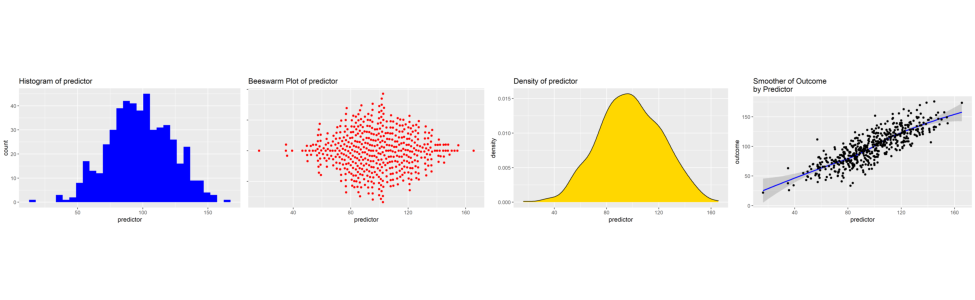
\includegraphics{introduction-to-ggplot2_files/figure-latex/unnamed-chunk-1-1.pdf}

\hypertarget{options-optional-titles-themes-etc.}{%
\subsection{\texorpdfstring{\textbf{options}: \emph{optional} titles,
themes,
etc.}{options: optional titles, themes, etc.}}\label{options-optional-titles-themes-etc.}}

\hypertarget{a-simple-quick-example}{%
\section{A Simple Quick Example}\label{a-simple-quick-example}}

The intent of this tutorial is to build the foundation of this idea
that:

\begin{quote}
A little bit of ggplot can go a long way
\end{quote}

and to give you a simple introduction to the idea that any ggplot graph
is composed of:

\begin{quote}
an \texttt{aesthetic} + \texttt{a\ geom\ or\ two} +
\texttt{other\ optional\ elements\ like\ titles\ and\ themes}.
\end{quote}

So, as a quick and simple example\ldots{}

\begin{Shaded}
\begin{Highlighting}[]
\KeywordTok{library}\NormalTok{(ggplot2)}

\KeywordTok{ggplot}\NormalTok{(my_demo_data, }\CommentTok{# the data that I am using}
       \KeywordTok{aes}\NormalTok{(}\DataTypeTok{x =}\NormalTok{ my_outcome)) }\OperatorTok{+}\StringTok{ }\CommentTok{# aesthetic: what I am graphing}
\StringTok{  }\KeywordTok{geom_histogram}\NormalTok{(}\DataTypeTok{fill =} \StringTok{"red"}\NormalTok{, }\CommentTok{# geom: how I am graphing it}
                 \DataTypeTok{color =} \StringTok{"black"}\NormalTok{) }\CommentTok{# options: fill = "red"; color = "black"}
\end{Highlighting}
\end{Shaded}

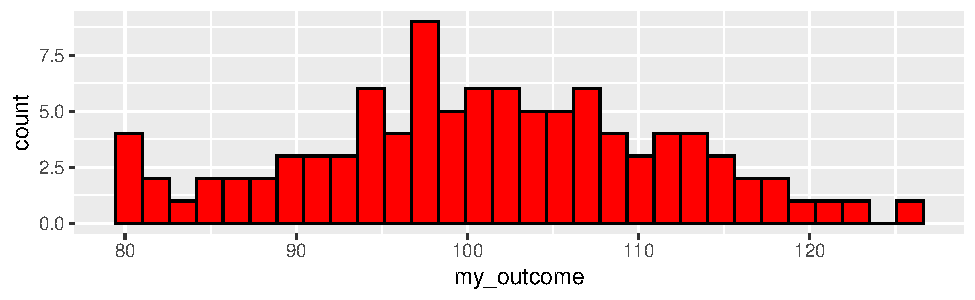
\includegraphics{introduction-to-ggplot2_files/figure-latex/unnamed-chunk-3-1.pdf}

And now, with labels\ldots{}

\begin{Shaded}
\begin{Highlighting}[]
\KeywordTok{ggplot}\NormalTok{(my_demo_data, }\CommentTok{# the data that I am using}
       \KeywordTok{aes}\NormalTok{(}\DataTypeTok{x =}\NormalTok{ my_outcome)) }\OperatorTok{+}\StringTok{ }\CommentTok{# aesthetic: what I am graphing}
\StringTok{  }\KeywordTok{geom_histogram}\NormalTok{(}\DataTypeTok{fill =} \StringTok{"red"}\NormalTok{, }\CommentTok{# geom: how I am graphing it}
                 \DataTypeTok{color =} \StringTok{"black"}\NormalTok{) }\OperatorTok{+}
\StringTok{  }\KeywordTok{labs}\NormalTok{(}\DataTypeTok{title =} \StringTok{"Your Title Here"}\NormalTok{,}
       \DataTypeTok{subtitle =} \StringTok{"Your Subtitle Here"}\NormalTok{,}
       \DataTypeTok{caption =} \StringTok{"A Caption, If You Want One"}\NormalTok{,}
       \DataTypeTok{x =} \StringTok{"my outcome"}\NormalTok{,}
       \DataTypeTok{y =} \StringTok{"count"}\NormalTok{)}
\end{Highlighting}
\end{Shaded}

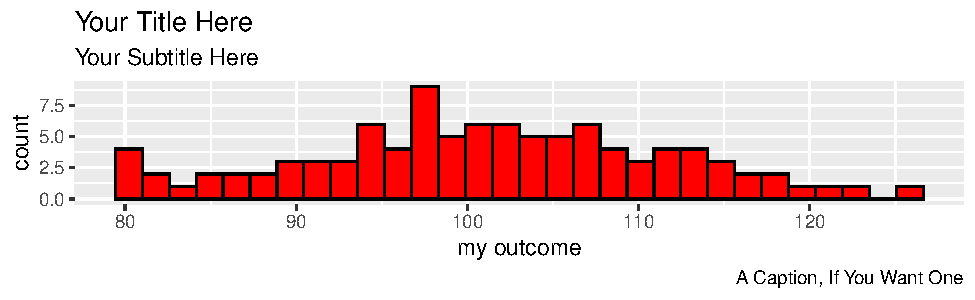
\includegraphics{introduction-to-ggplot2_files/figure-latex/unnamed-chunk-4-1.pdf}

This document is a \emph{very brief} introduction to the \emph{basic}
ideas of ggplot2. More information about ggplot can be found
\href{http://ggplot2.org/}{here}. More ggplot2 examples can be found
\href{http://www-personal.umich.edu/~agrogan/how_to_choose_a_chart/how_to_choose_a_chart_v3.html}{here}.

\hypertarget{call-the-relevant-libraries}{%
\section{Call The Relevant
Libraries}\label{call-the-relevant-libraries}}

You will need a few
\href{http://www-personal.umich.edu/~agrogan/R/introduction-to-R.html\#2_base_r_and_libraries}{R
libraries} to work in ggplot. You may \emph{only} need
\texttt{library(ggplot2)}, but some of these other libraries may also be
helpful.

\begin{Shaded}
\begin{Highlighting}[]
\KeywordTok{library}\NormalTok{(ggplot2) }\CommentTok{# beautiful graphs}

\KeywordTok{library}\NormalTok{(ggthemes) }\CommentTok{# nice themes for ggplot2}

\KeywordTok{library}\NormalTok{(ggbeeswarm) }\CommentTok{# "beeswarm" plots}

\KeywordTok{library}\NormalTok{(cowplot) }\CommentTok{# arrrange graphs}

\KeywordTok{library}\NormalTok{(pander) }\CommentTok{# nice tables}

\KeywordTok{library}\NormalTok{(psych) }\CommentTok{# nice table of descriptive statistics}
\end{Highlighting}
\end{Shaded}

\hypertarget{simulated-data}{%
\section{Simulated Data}\label{simulated-data}}

In this example, we simulate some data. But your own learning of ggplot
will progress more quickly if you use data that you have access to, on
an issue that you care about.

Here are the first few rows of simulated data:

\begin{longtable}[]{@{}ccc@{}}
\toprule
\begin{minipage}[b]{0.15\columnwidth}\centering
predictor\strut
\end{minipage} & \begin{minipage}[b]{0.13\columnwidth}\centering
outcome\strut
\end{minipage} & \begin{minipage}[b]{0.13\columnwidth}\centering
group\strut
\end{minipage}\tabularnewline
\midrule
\endhead
\begin{minipage}[t]{0.15\columnwidth}\centering
105.5\strut
\end{minipage} & \begin{minipage}[t]{0.13\columnwidth}\centering
108.3\strut
\end{minipage} & \begin{minipage}[t]{0.13\columnwidth}\centering
1\strut
\end{minipage}\tabularnewline
\begin{minipage}[t]{0.15\columnwidth}\centering
135.4\strut
\end{minipage} & \begin{minipage}[t]{0.13\columnwidth}\centering
154.9\strut
\end{minipage} & \begin{minipage}[t]{0.13\columnwidth}\centering
1\strut
\end{minipage}\tabularnewline
\begin{minipage}[t]{0.15\columnwidth}\centering
144.4\strut
\end{minipage} & \begin{minipage}[t]{0.13\columnwidth}\centering
166.6\strut
\end{minipage} & \begin{minipage}[t]{0.13\columnwidth}\centering
1\strut
\end{minipage}\tabularnewline
\begin{minipage}[t]{0.15\columnwidth}\centering
88.69\strut
\end{minipage} & \begin{minipage}[t]{0.13\columnwidth}\centering
67.91\strut
\end{minipage} & \begin{minipage}[t]{0.13\columnwidth}\centering
0\strut
\end{minipage}\tabularnewline
\begin{minipage}[t]{0.15\columnwidth}\centering
87.34\strut
\end{minipage} & \begin{minipage}[t]{0.13\columnwidth}\centering
74.28\strut
\end{minipage} & \begin{minipage}[t]{0.13\columnwidth}\centering
1\strut
\end{minipage}\tabularnewline
\begin{minipage}[t]{0.15\columnwidth}\centering
98.74\strut
\end{minipage} & \begin{minipage}[t]{0.13\columnwidth}\centering
82.44\strut
\end{minipage} & \begin{minipage}[t]{0.13\columnwidth}\centering
0\strut
\end{minipage}\tabularnewline
\begin{minipage}[t]{0.15\columnwidth}\centering
116.6\strut
\end{minipage} & \begin{minipage}[t]{0.13\columnwidth}\centering
102.8\strut
\end{minipage} & \begin{minipage}[t]{0.13\columnwidth}\centering
0\strut
\end{minipage}\tabularnewline
\begin{minipage}[t]{0.15\columnwidth}\centering
89.86\strut
\end{minipage} & \begin{minipage}[t]{0.13\columnwidth}\centering
74.61\strut
\end{minipage} & \begin{minipage}[t]{0.13\columnwidth}\centering
0\strut
\end{minipage}\tabularnewline
\begin{minipage}[t]{0.15\columnwidth}\centering
108.2\strut
\end{minipage} & \begin{minipage}[t]{0.13\columnwidth}\centering
102.9\strut
\end{minipage} & \begin{minipage}[t]{0.13\columnwidth}\centering
1\strut
\end{minipage}\tabularnewline
\begin{minipage}[t]{0.15\columnwidth}\centering
91.8\strut
\end{minipage} & \begin{minipage}[t]{0.13\columnwidth}\centering
117.4\strut
\end{minipage} & \begin{minipage}[t]{0.13\columnwidth}\centering
0\strut
\end{minipage}\tabularnewline
\bottomrule
\end{longtable}

\hypertarget{the-essential-idea-of-ggplot2-is-simple.}{%
\section{\texorpdfstring{The Essential Idea Of \texttt{ggplot2} Is
Simple.}{The Essential Idea Of ggplot2 Is Simple.}}\label{the-essential-idea-of-ggplot2-is-simple.}}

There are 3 essential elements to any ggplot call:

\begin{enumerate}
\def\labelenumi{\arabic{enumi}.}
\tightlist
\item
  An \emph{aesthetic} that tells ggplot which variables are being mapped
  to the \emph{x axis}, \emph{y axis}, (and often other attributes of
  the graph, such as the \emph{color fill}). Intuitively, the aesthetic
  can be thought of as \emph{what you are graphing}.
\item
  A \emph{geom} or \emph{geometry} that tells ggplot about the basic
  structure of the graph. Intuitively, the geom can be thought of as
  \emph{how you are graphing it}.
\item
  Other options, such as a \emph{graph title}, \emph{axis labels} and
  \emph{overall theme} for the graph.
\end{enumerate}

\hypertarget{ggplot2-starts-by-calling-the-aesthetic}{%
\subsection{\texorpdfstring{ggplot2 Starts By Calling The
\texttt{aes}thetic}{ggplot2 Starts By Calling The aesthetic}}\label{ggplot2-starts-by-calling-the-aesthetic}}

For one variable:

\texttt{p\ \textless{}-\ ggplot(mydata,\ aes(x\ =\ ...))} This says
there is only one variable running along the horizontal \emph{x} axis in
the aesthetic.

\begin{quote}
The \texttt{p\ \textless{}-...} means that we are \emph{assigning} this
graph aesthetic to plot \emph{p}. We can then add other features to plot
\emph{p} as we continue our work. This \emph{iterative} nature of
\texttt{ggplot2} is one of the things that makes it so powerful. As your
workflow and your documents become more complex, you can build a simple
consistent foundation\footnote{By way of illustration, this foundation
  could be just an aesthetic (e.g. \texttt{aes(...)}) alone, or possibly
  an aesthetic plus a theme (e.g. \texttt{theme\_tufte()}), plus axis
  labels to create a consistent look and feel for your graphs across a
  report.} for your graphs, then add something simple to make a first
graph, and a different something simple to make a second graph.
\end{quote}

For two variables:

\texttt{p\ \textless{}-\ ggplot(mydata,\ aes(x\ =\ ...,\ y\ =\ ...))}
This says there are two variables: one for the horizontal \emph{x} axis;
and another for the vertical \emph{y} axis, in the aesthetic.

\hypertarget{we-then-call-the-geometry}{%
\subsection{\texorpdfstring{We Then Call The
\texttt{geom}etry}{We Then Call The geometry}}\label{we-then-call-the-geometry}}

We can then add different geometries to our plot:

For one variable:

\texttt{+\ geom\_density()} This says add a density geometry to the
graph.

\texttt{+\ geom\_histogram()} This says add a histogram geometry to the
graph.

\texttt{+\ geom\_violin()} This says add a \emph{violin plot} geometry
to the graph.

\texttt{+\ geom\_beeswarm()} This says add a \emph{beeswarm} geometry to
the graph.

\begin{quote}
A \emph{beeswarm} is a creative layout of points that intuitively lets
you understand the distribution of a quantity. The \emph{beeswarm}
geometry requires separate installation of the \texttt{ggbeeswarm}
package. You also need to call \texttt{library(ggbeeswarm)} to use this
geometry.
\end{quote}

For two variables:

\texttt{+\ geom\_point()} This says add a point (scatterplot) geometry
to the graph.

\texttt{+\ geom\_smooth()} This says add a smoother to the graph.

\hypertarget{examples}{%
\section{Examples}\label{examples}}

\hypertarget{one-continuous-variable-at-a-time}{%
\subsection{One Continuous Variable At A
Time}\label{one-continuous-variable-at-a-time}}

\hypertarget{dotplot}{%
\subsubsection{Dotplot}\label{dotplot}}

\begin{Shaded}
\begin{Highlighting}[]
\CommentTok{# call ggplot2 where aesthetic is: x uses our predictor variable}

\NormalTok{p1 <-}\StringTok{ }\KeywordTok{ggplot}\NormalTok{(mydata, }
             \KeywordTok{aes}\NormalTok{(}\DataTypeTok{x =}\NormalTok{ predictor)) }
\end{Highlighting}
\end{Shaded}

\begin{Shaded}
\begin{Highlighting}[]
\NormalTok{p1 }\OperatorTok{+}\StringTok{ }
\StringTok{  }\KeywordTok{geom_dotplot}\NormalTok{(}\DataTypeTok{dotsize =} \FloatTok{.15}\NormalTok{) }\CommentTok{# add dotplot geom}
\end{Highlighting}
\end{Shaded}

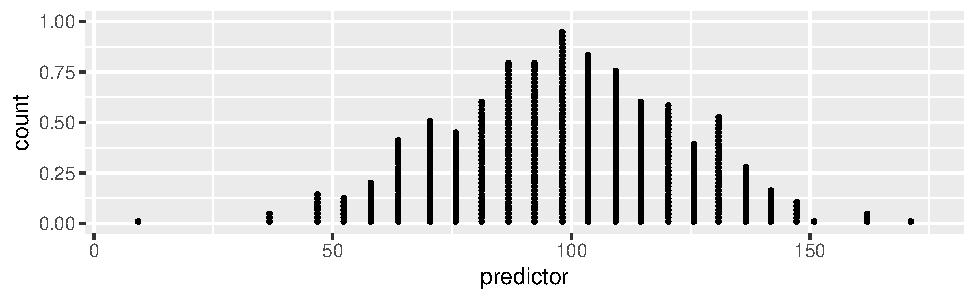
\includegraphics{introduction-to-ggplot2_files/figure-latex/unnamed-chunk-7-1.pdf}

\hypertarget{add-some-options}{%
\subsubsection{Add Some Options}\label{add-some-options}}

\begin{Shaded}
\begin{Highlighting}[]
\NormalTok{p1 }\OperatorTok{+}\StringTok{ }
\StringTok{  }\KeywordTok{geom_dotplot}\NormalTok{(}\DataTypeTok{dotsize =} \FloatTok{.15}\NormalTok{, }
               \DataTypeTok{fill=}\StringTok{"red"}\NormalTok{) }\OperatorTok{+}\StringTok{ }\CommentTok{# add dotplot geom in red}
\StringTok{  }\KeywordTok{labs}\NormalTok{(}\DataTypeTok{title =}\StringTok{"Dotplot of predictor"}\NormalTok{) }\CommentTok{# Add title}
\end{Highlighting}
\end{Shaded}

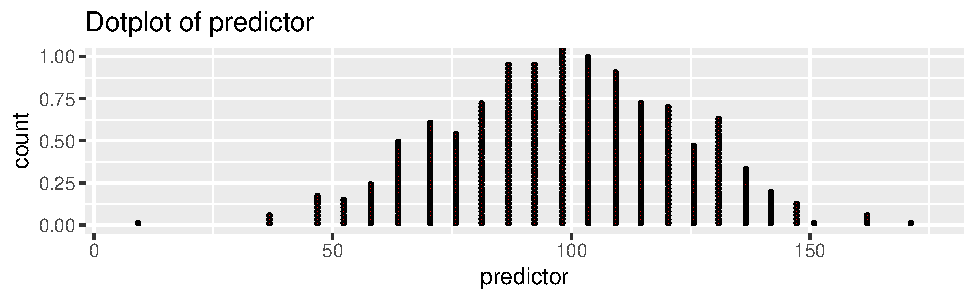
\includegraphics{introduction-to-ggplot2_files/figure-latex/unnamed-chunk-8-1.pdf}

\hypertarget{different-geoms}{%
\subsubsection{Different Geoms}\label{different-geoms}}

\hypertarget{histogram}{%
\paragraph{Histogram}\label{histogram}}

\begin{Shaded}
\begin{Highlighting}[]
\NormalTok{p1 }\OperatorTok{+}\StringTok{ }\KeywordTok{geom_histogram}\NormalTok{(}\DataTypeTok{fill =} \StringTok{"blue"}\NormalTok{, }
                    \DataTypeTok{color=}\StringTok{"black"}\NormalTok{) }\OperatorTok{+}\StringTok{ }\CommentTok{# add histogram geom in blue}
\StringTok{  }\KeywordTok{labs}\NormalTok{(}\DataTypeTok{title =}\StringTok{"Histogram of predictor"}\NormalTok{) }\CommentTok{# Add title}
\end{Highlighting}
\end{Shaded}

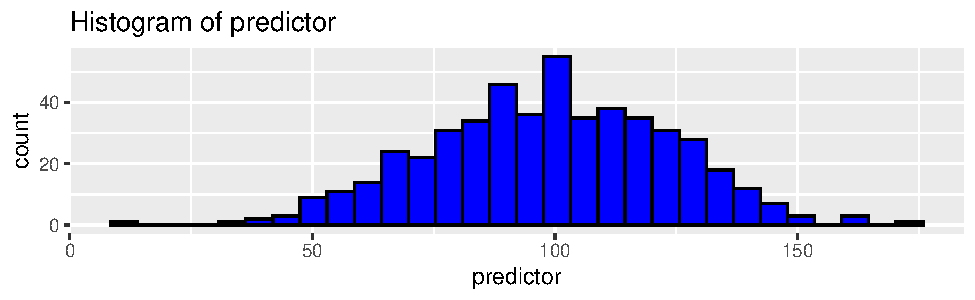
\includegraphics{introduction-to-ggplot2_files/figure-latex/unnamed-chunk-9-1.pdf}

\hypertarget{density}{%
\paragraph{Density}\label{density}}

\begin{Shaded}
\begin{Highlighting}[]
\NormalTok{p1 }\OperatorTok{+}\StringTok{ }\KeywordTok{geom_density}\NormalTok{(}\DataTypeTok{fill =} \StringTok{"gold"}\NormalTok{) }\OperatorTok{+}\StringTok{ }\CommentTok{# add density geom in gold}
\StringTok{  }\KeywordTok{labs}\NormalTok{(}\DataTypeTok{title =}\StringTok{"Density of predictor"}\NormalTok{) }\CommentTok{# Add title}
\end{Highlighting}
\end{Shaded}

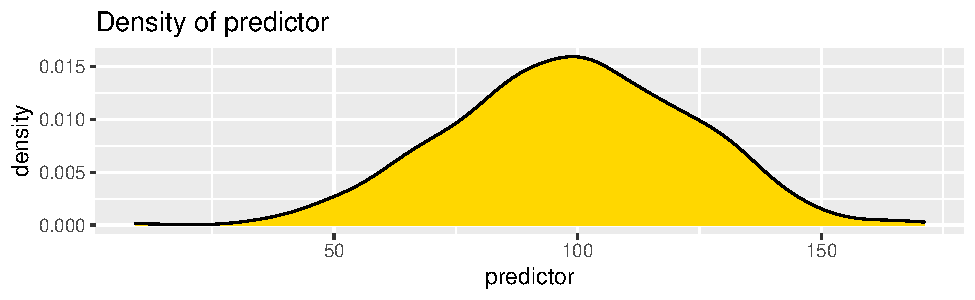
\includegraphics{introduction-to-ggplot2_files/figure-latex/unnamed-chunk-10-1.pdf}

\hypertarget{violin-plot}{%
\paragraph{Violin Plot}\label{violin-plot}}

\begin{Shaded}
\begin{Highlighting}[]
\NormalTok{p2 <-}\StringTok{ }\KeywordTok{ggplot}\NormalTok{(mydata, }
             \KeywordTok{aes}\NormalTok{(}\DataTypeTok{x =} \DecValTok{1}\NormalTok{, }\CommentTok{# we need an aesthetic with _x_}
                 \DataTypeTok{y =}\NormalTok{ predictor)) }\CommentTok{# & _y_}

\NormalTok{p2 }\OperatorTok{+}\StringTok{ }\KeywordTok{geom_violin}\NormalTok{(}\DataTypeTok{fill =} \StringTok{"purple"}\NormalTok{) }\OperatorTok{+}
\StringTok{  }\KeywordTok{labs}\NormalTok{(}\DataTypeTok{title =}\StringTok{"Violin Plot of predictor"}\NormalTok{) }\CommentTok{# Add title}
\end{Highlighting}
\end{Shaded}

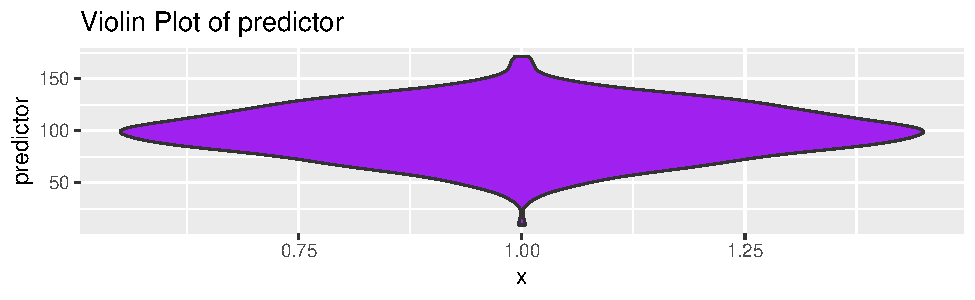
\includegraphics{introduction-to-ggplot2_files/figure-latex/unnamed-chunk-11-1.pdf}

\hypertarget{beeswarm}{%
\paragraph{Beeswarm}\label{beeswarm}}

\begin{Shaded}
\begin{Highlighting}[]
\NormalTok{p3 <-}\StringTok{ }\KeywordTok{ggplot}\NormalTok{(mydata, }
             \KeywordTok{aes}\NormalTok{(}\DataTypeTok{x =}\NormalTok{ predictor, }\CommentTok{# we need an aesthetic with _x_}
                 \DataTypeTok{y =} \DecValTok{1}\NormalTok{)) }\CommentTok{# & _y_}

\NormalTok{p3 }\OperatorTok{+}\StringTok{ }\KeywordTok{geom_beeswarm}\NormalTok{(}\DataTypeTok{color =} \StringTok{"red"}\NormalTok{, }
                   \DataTypeTok{groupOnX =} \OtherTok{FALSE}\NormalTok{) }\OperatorTok{+}
\StringTok{  }\KeywordTok{labs}\NormalTok{(}\DataTypeTok{title =} \StringTok{"Beeswarm Plot of predictor"}\NormalTok{) }\OperatorTok{+}\StringTok{ }\CommentTok{# Add title}
\StringTok{  }\KeywordTok{theme}\NormalTok{(}\DataTypeTok{axis.title.y =} \KeywordTok{element_blank}\NormalTok{(), }
        \DataTypeTok{axis.text.y =} \KeywordTok{element_blank}\NormalTok{()) }\CommentTok{# tweak y axis}
\end{Highlighting}
\end{Shaded}

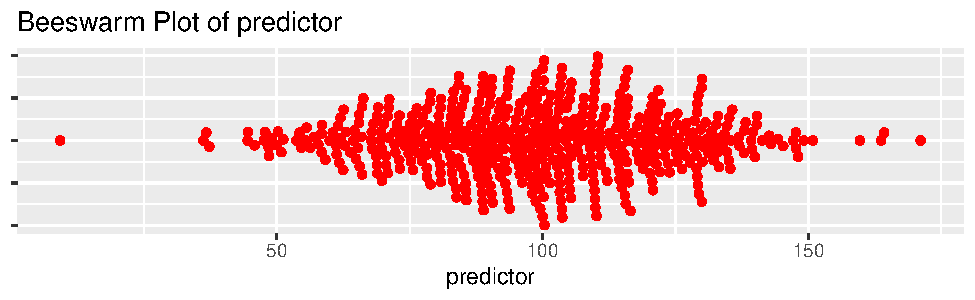
\includegraphics{introduction-to-ggplot2_files/figure-latex/unnamed-chunk-12-1.pdf}

\hypertarget{one-categorical-variable-at-a-time}{%
\subsection{One Categorical Variable at a
Time}\label{one-categorical-variable-at-a-time}}

The easiest way to represent a single categorical variable is likely a
bar graph.

\begin{quote}
Here bars represent the \textbf{count} of observations in each group.
\end{quote}

\begin{Shaded}
\begin{Highlighting}[]
\NormalTok{p_barchart <-}\StringTok{ }\KeywordTok{ggplot}\NormalTok{(mydata,}
                     \KeywordTok{aes}\NormalTok{(}\DataTypeTok{x =}\NormalTok{ group)) }\OperatorTok{+}
\StringTok{  }\KeywordTok{geom_bar}\NormalTok{(}\DataTypeTok{fill =} \StringTok{"red"}\NormalTok{) }

\NormalTok{p_barchart}
\end{Highlighting}
\end{Shaded}

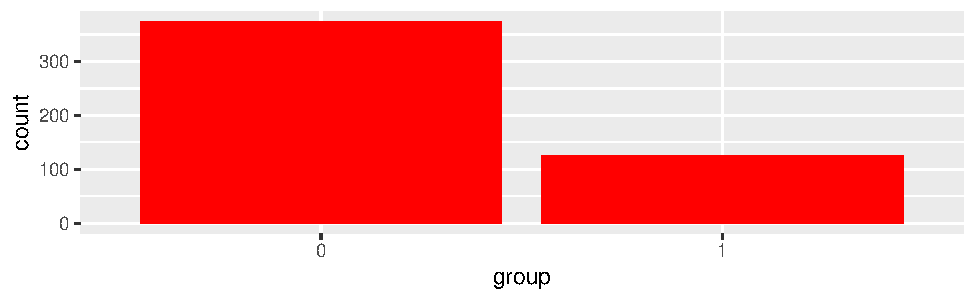
\includegraphics{introduction-to-ggplot2_files/figure-latex/unnamed-chunk-13-1.pdf}

\begin{quote}
Changing the \emph{aesthetic} slightly results in a \emph{stacked} bar
chart. Since all groups are stacked in 1 bar, we have to add information
about the colors that we want to use to distinguish the groups.
\end{quote}

\begin{Shaded}
\begin{Highlighting}[]
\NormalTok{p_stacked_barchart <-}\StringTok{ }\KeywordTok{ggplot}\NormalTok{(mydata, }
                             \KeywordTok{aes}\NormalTok{(}\DataTypeTok{x =} \DecValTok{1}\NormalTok{,}
                                 \DataTypeTok{fill =}\NormalTok{ group)) }\OperatorTok{+}
\StringTok{  }\KeywordTok{geom_bar}\NormalTok{() }\OperatorTok{+}
\StringTok{  }\KeywordTok{scale_fill_manual}\NormalTok{(}\DataTypeTok{values =} \KeywordTok{c}\NormalTok{(}\StringTok{"red"}\NormalTok{, }\StringTok{"blue"}\NormalTok{))}

\NormalTok{p_stacked_barchart}
\end{Highlighting}
\end{Shaded}

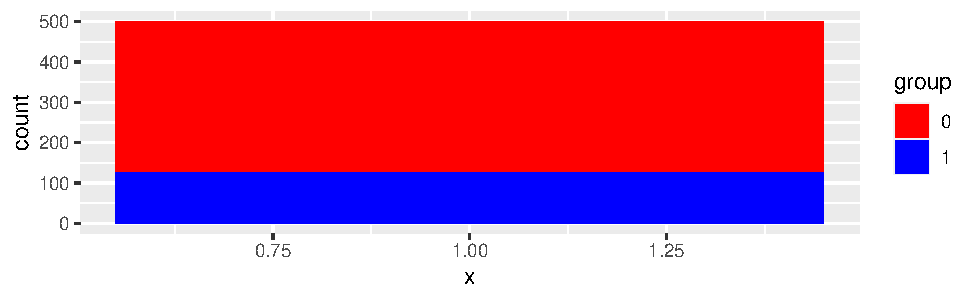
\includegraphics{introduction-to-ggplot2_files/figure-latex/unnamed-chunk-14-1.pdf}

\hypertarget{a-categorical-variable-and-a-continuous-variable}{%
\subsection{A Categorical Variable and A Continuous
Variable}\label{a-categorical-variable-and-a-continuous-variable}}

\hypertarget{barchart}{%
\subsubsection{Barchart}\label{barchart}}

\begin{quote}
Here bars represent the \textbf{average value of our outcome variable}
for members of each group.
\end{quote}

\begin{Shaded}
\begin{Highlighting}[]
\NormalTok{p_barchart_of_mean <-}\StringTok{ }\KeywordTok{ggplot}\NormalTok{(mydata, }
                             \KeywordTok{aes}\NormalTok{(}\DataTypeTok{x =}\NormalTok{ group, }\CommentTok{# slightly different aesthetic}
                                 \DataTypeTok{y =}\NormalTok{ outcome)) }\OperatorTok{+}\StringTok{ }
\StringTok{  }\KeywordTok{stat_summary}\NormalTok{(}\DataTypeTok{fun.y =}\NormalTok{ mean, }\CommentTok{# take the mean of the data}
               \DataTypeTok{fill =} \StringTok{"blue"}\NormalTok{, }\CommentTok{# fill color}
               \DataTypeTok{geom =} \StringTok{"bar"}\NormalTok{) }\CommentTok{# we want to summarize data with bars}

\NormalTok{p_barchart_of_mean}
\end{Highlighting}
\end{Shaded}

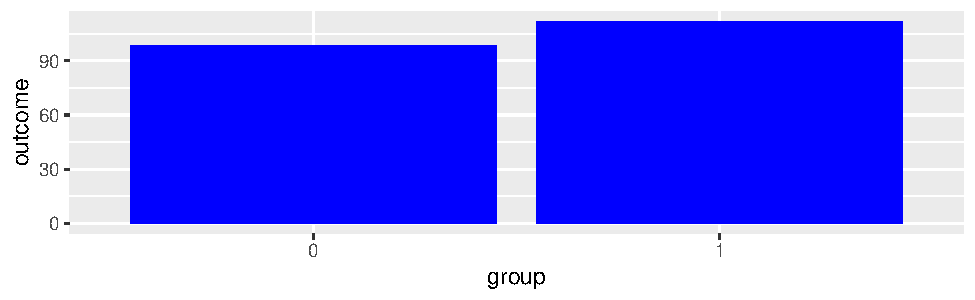
\includegraphics{introduction-to-ggplot2_files/figure-latex/unnamed-chunk-15-1.pdf}

\hypertarget{two-continuous-variables-at-a-time}{%
\subsection{Two Continuous Variables At A
Time}\label{two-continuous-variables-at-a-time}}

\hypertarget{basic-scatterplot}{%
\subsubsection{Basic Scatterplot}\label{basic-scatterplot}}

\begin{Shaded}
\begin{Highlighting}[]
\CommentTok{# call ggplot2 where aesthetic uses both predictor and outcome}

\NormalTok{p4 <-}\StringTok{ }\KeywordTok{ggplot}\NormalTok{(mydata, }
             \KeywordTok{aes}\NormalTok{(}\DataTypeTok{x =}\NormalTok{ predictor, }
                 \DataTypeTok{y =}\NormalTok{ outcome)) }\CommentTok{# set up aesthetic}

\NormalTok{p4 }\OperatorTok{+}\StringTok{ }\KeywordTok{geom_point}\NormalTok{() }\CommentTok{# add point geom (scatterplot)}
\end{Highlighting}
\end{Shaded}

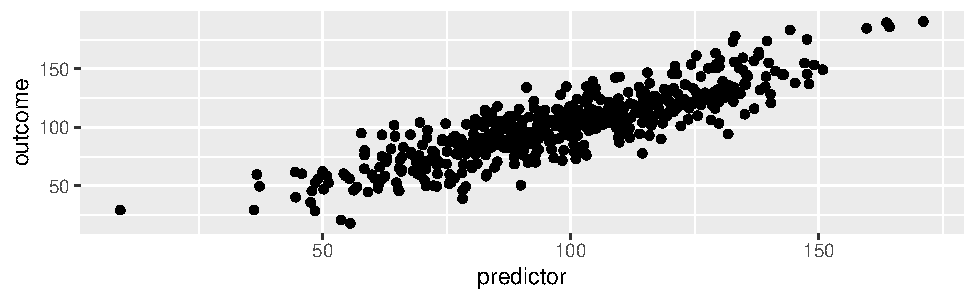
\includegraphics{introduction-to-ggplot2_files/figure-latex/unnamed-chunk-16-1.pdf}

\hypertarget{add-some-options-1}{%
\subsubsection{Add Some Options}\label{add-some-options-1}}

\begin{Shaded}
\begin{Highlighting}[]
\NormalTok{p4 }\OperatorTok{+}\StringTok{ }\CommentTok{# start with basic plot that has only an aesthetic}
\StringTok{  }\KeywordTok{geom_point}\NormalTok{(}\DataTypeTok{color =} \StringTok{"blue"}\NormalTok{) }\OperatorTok{+}\StringTok{ }\CommentTok{# add point geom in blue}
\StringTok{  }\KeywordTok{labs}\NormalTok{(}\DataTypeTok{title =}\StringTok{"Scatterplot of Outcome by Predictor"}\NormalTok{) }\CommentTok{# add title}
\end{Highlighting}
\end{Shaded}

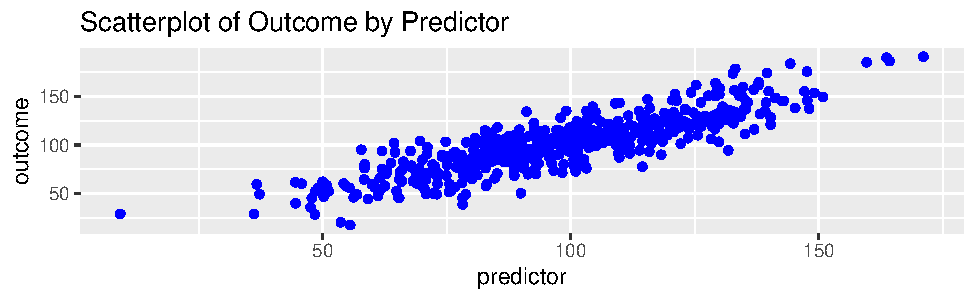
\includegraphics{introduction-to-ggplot2_files/figure-latex/unnamed-chunk-17-1.pdf}

\hypertarget{try-a-smoother}{%
\subsubsection{Try A Smoother}\label{try-a-smoother}}

\begin{Shaded}
\begin{Highlighting}[]
\NormalTok{p4 }\OperatorTok{+}\StringTok{ }
\StringTok{  }\KeywordTok{geom_smooth}\NormalTok{() }\OperatorTok{+}\StringTok{ }\CommentTok{# add smooth geom}
\StringTok{  }\KeywordTok{labs}\NormalTok{(}\DataTypeTok{title =}\StringTok{"Smoother of Outcome by Predictor"}\NormalTok{) }\CommentTok{# add title}
\end{Highlighting}
\end{Shaded}

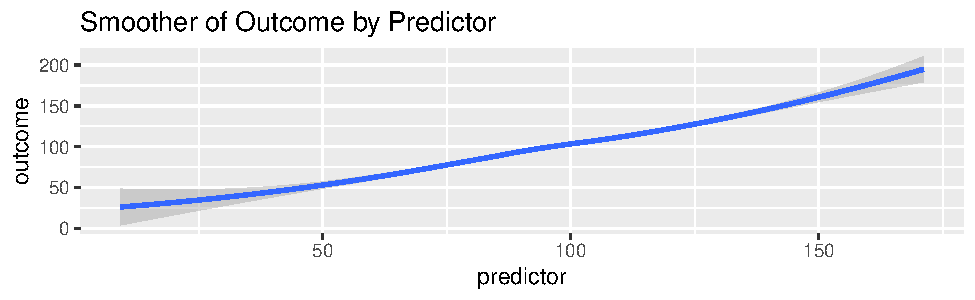
\includegraphics{introduction-to-ggplot2_files/figure-latex/unnamed-chunk-18-1.pdf}

\hypertarget{try-a-density-plot}{%
\subsubsection{Try A Density Plot}\label{try-a-density-plot}}

\hypertarget{simple-density}{%
\paragraph{Simple Density}\label{simple-density}}

\begin{Shaded}
\begin{Highlighting}[]
\NormalTok{p4 }\OperatorTok{+}\StringTok{ }
\StringTok{  }\KeywordTok{geom_density2d}\NormalTok{(}\DataTypeTok{color =} \StringTok{"blue"}\NormalTok{) }\OperatorTok{+}\StringTok{ }\CommentTok{# add density geom }
\StringTok{  }\KeywordTok{labs}\NormalTok{(}\DataTypeTok{title =}\StringTok{"Density Plot of Outcome by Predictor"}\NormalTok{) }\CommentTok{# add title}
\end{Highlighting}
\end{Shaded}

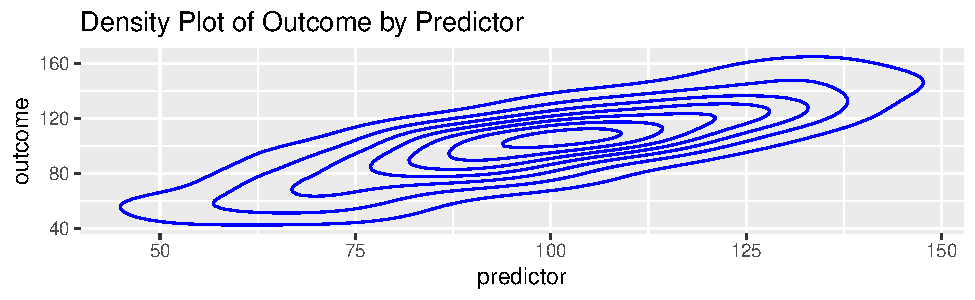
\includegraphics{introduction-to-ggplot2_files/figure-latex/unnamed-chunk-19-1.pdf}

\hypertarget{filled-density}{%
\paragraph{Filled Density}\label{filled-density}}

\begin{quote}
While not strictly necessary, the use of \texttt{scale\_fill\_gradient}
seems to improve the presentation. You can choose your own colors.
\end{quote}

\begin{Shaded}
\begin{Highlighting}[]
\NormalTok{p4 }\OperatorTok{+}\StringTok{ }
\StringTok{  }\KeywordTok{stat_density_2d}\NormalTok{(}\KeywordTok{aes}\NormalTok{(}\DataTypeTok{fill =}\NormalTok{ ..level..), }
                  \DataTypeTok{geom =} \StringTok{"polygon"}\NormalTok{) }\OperatorTok{+}\StringTok{ }\CommentTok{# add filled density geom }
\StringTok{  }\KeywordTok{scale_fill_gradient}\NormalTok{(}\DataTypeTok{low =} \StringTok{"blue"}\NormalTok{,}
                      \DataTypeTok{high =} \StringTok{"red"}\NormalTok{) }\OperatorTok{+}
\StringTok{  }\KeywordTok{labs}\NormalTok{(}\DataTypeTok{title =}\StringTok{"Density Plot of Outcome by Predictor"}\NormalTok{) }\CommentTok{# add title}
\end{Highlighting}
\end{Shaded}

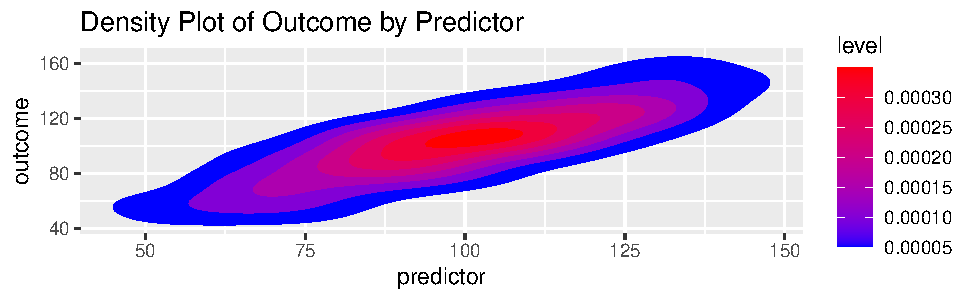
\includegraphics{introduction-to-ggplot2_files/figure-latex/unnamed-chunk-20-1.pdf}

\hypertarget{add-points}{%
\paragraph{Add Points}\label{add-points}}

\begin{Shaded}
\begin{Highlighting}[]
\NormalTok{p4 }\OperatorTok{+}\StringTok{ }
\StringTok{  }\KeywordTok{stat_density_2d}\NormalTok{(}\KeywordTok{aes}\NormalTok{(}\DataTypeTok{fill =}\NormalTok{ ..level..), }
                  \DataTypeTok{geom =} \StringTok{"polygon"}\NormalTok{) }\OperatorTok{+}\StringTok{ }\CommentTok{# add filled density geom}
\StringTok{  }\KeywordTok{geom_point}\NormalTok{(}\DataTypeTok{color =} \StringTok{"orange"}\NormalTok{) }\OperatorTok{+}
\StringTok{    }\KeywordTok{scale_fill_gradient}\NormalTok{(}\DataTypeTok{low =} \StringTok{"blue"}\NormalTok{,}
                      \DataTypeTok{high =} \StringTok{"red"}\NormalTok{) }\OperatorTok{+}
\StringTok{  }\KeywordTok{labs}\NormalTok{(}\DataTypeTok{title =}\StringTok{"Density Plot of Outcome by Predictor"}\NormalTok{) }\CommentTok{# add title}
\end{Highlighting}
\end{Shaded}

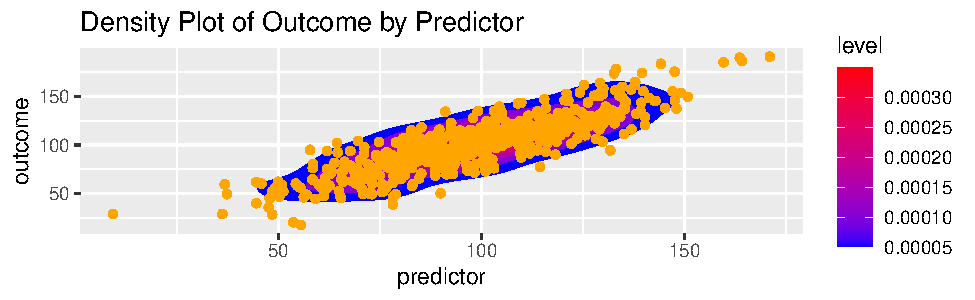
\includegraphics{introduction-to-ggplot2_files/figure-latex/unnamed-chunk-21-1.pdf}

\hypertarget{use-a-raster-geom-instead}{%
\paragraph{Use a Raster Geom Instead}\label{use-a-raster-geom-instead}}

\begin{Shaded}
\begin{Highlighting}[]
\NormalTok{p4 }\OperatorTok{+}\StringTok{ }
\StringTok{  }\KeywordTok{stat_density_2d}\NormalTok{(}\DataTypeTok{geom =} \StringTok{"raster"}\NormalTok{, }
                  \KeywordTok{aes}\NormalTok{(}\DataTypeTok{fill =}\NormalTok{ ..density..),}
                  \DataTypeTok{contour =} \OtherTok{FALSE}\NormalTok{) }\OperatorTok{+}
\StringTok{  }\KeywordTok{scale_fill_gradient}\NormalTok{(}\DataTypeTok{low =} \StringTok{"blue"}\NormalTok{,}
                      \DataTypeTok{high =} \StringTok{"red"}\NormalTok{) }\OperatorTok{+}
\StringTok{  }\KeywordTok{labs}\NormalTok{(}\DataTypeTok{title =}\StringTok{"Density Plot (Raster) of Outcome by Predictor"}\NormalTok{) }\CommentTok{# add title}
\end{Highlighting}
\end{Shaded}

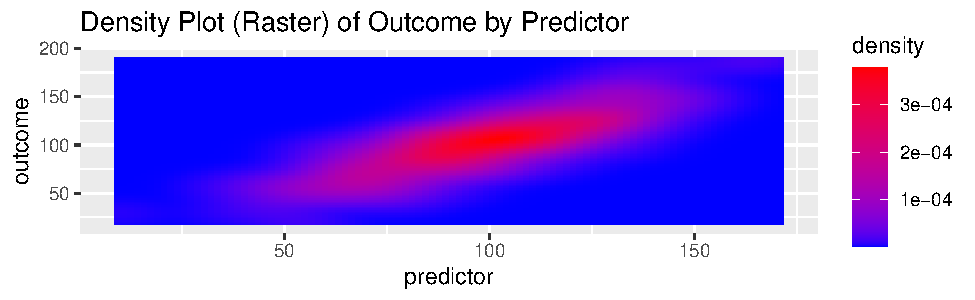
\includegraphics{introduction-to-ggplot2_files/figure-latex/unnamed-chunk-22-1.pdf}

\hypertarget{try-a-hexagon-geom}{%
\subsubsection{Try a Hexagon Geom}\label{try-a-hexagon-geom}}

\texttt{geom\_hex} may be a useful visualization, especially when there
is the possiblity of \emph{over-plotting} due to many many points.

\begin{Shaded}
\begin{Highlighting}[]
\NormalTok{p4 }\OperatorTok{+}\StringTok{ }
\StringTok{  }\KeywordTok{geom_hex}\NormalTok{() }\OperatorTok{+}
\StringTok{   }\KeywordTok{scale_fill_gradient}\NormalTok{(}\DataTypeTok{low =} \StringTok{"blue"}\NormalTok{,}
                      \DataTypeTok{high =} \StringTok{"red"}\NormalTok{) }\OperatorTok{+}
\StringTok{  }\KeywordTok{labs}\NormalTok{(}\DataTypeTok{title =}\StringTok{"Hexagon Plot of Outcome by Predictor"}\NormalTok{) }\CommentTok{# add title}
\end{Highlighting}
\end{Shaded}

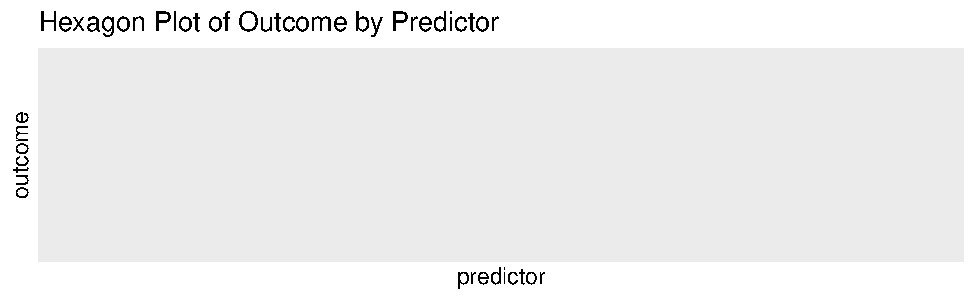
\includegraphics{introduction-to-ggplot2_files/figure-latex/unnamed-chunk-23-1.pdf}

\hypertarget{combine-points-and-smoother-and-add-some-themes}{%
\subsubsection{Combine Points and Smoother And Add Some
Themes}\label{combine-points-and-smoother-and-add-some-themes}}

\hypertarget{themes-included-with-ggplot2}{%
\paragraph{\texorpdfstring{Themes Included With
\texttt{ggplot2}}{Themes Included With ggplot2}}\label{themes-included-with-ggplot2}}

\hypertarget{default-ggplot2-theme}{%
\subparagraph{Default ggplot2 Theme}\label{default-ggplot2-theme}}

\begin{Shaded}
\begin{Highlighting}[]
\NormalTok{p4 }\OperatorTok{+}\StringTok{ }
\StringTok{  }\KeywordTok{geom_point}\NormalTok{() }\OperatorTok{+}\StringTok{ }\CommentTok{# point geom}
\StringTok{  }\KeywordTok{geom_smooth}\NormalTok{() }\OperatorTok{+}\StringTok{ }\CommentTok{# add smooth geom}
\StringTok{  }\KeywordTok{labs}\NormalTok{(}\DataTypeTok{title =}\StringTok{"Scatterplot And Smoother of Outcome"}\NormalTok{, }
       \DataTypeTok{subtitle =} \StringTok{"nby Predictor"}\NormalTok{) }\OperatorTok{+}\StringTok{ }\CommentTok{# add title}
\StringTok{  }\KeywordTok{theme_grey}\NormalTok{() }\CommentTok{# default theme}
\end{Highlighting}
\end{Shaded}

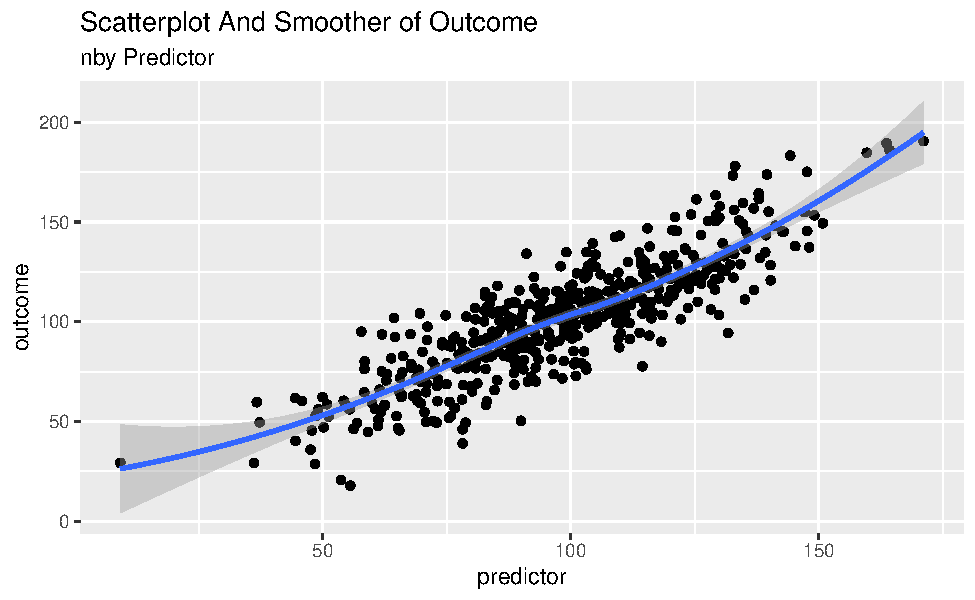
\includegraphics{introduction-to-ggplot2_files/figure-latex/unnamed-chunk-24-1.pdf}

\hypertarget{the-minimal-theme}{%
\subparagraph{The ``minimal'' theme}\label{the-minimal-theme}}

\begin{Shaded}
\begin{Highlighting}[]
\NormalTok{p4 }\OperatorTok{+}\StringTok{ }
\StringTok{  }\KeywordTok{geom_point}\NormalTok{() }\OperatorTok{+}\StringTok{ }\CommentTok{# point geom}
\StringTok{  }\KeywordTok{geom_smooth}\NormalTok{() }\OperatorTok{+}\StringTok{ }\CommentTok{# add smooth geom}
\StringTok{  }\KeywordTok{labs}\NormalTok{(}\DataTypeTok{title =}\StringTok{"Scatterplot And Smoother of Outcome }\CharTok{\textbackslash{}n}\StringTok{by Predictor"}\NormalTok{) }\OperatorTok{+}\StringTok{ }\CommentTok{# add title}
\StringTok{  }\KeywordTok{theme_minimal}\NormalTok{() }\CommentTok{# default theme}
\end{Highlighting}
\end{Shaded}

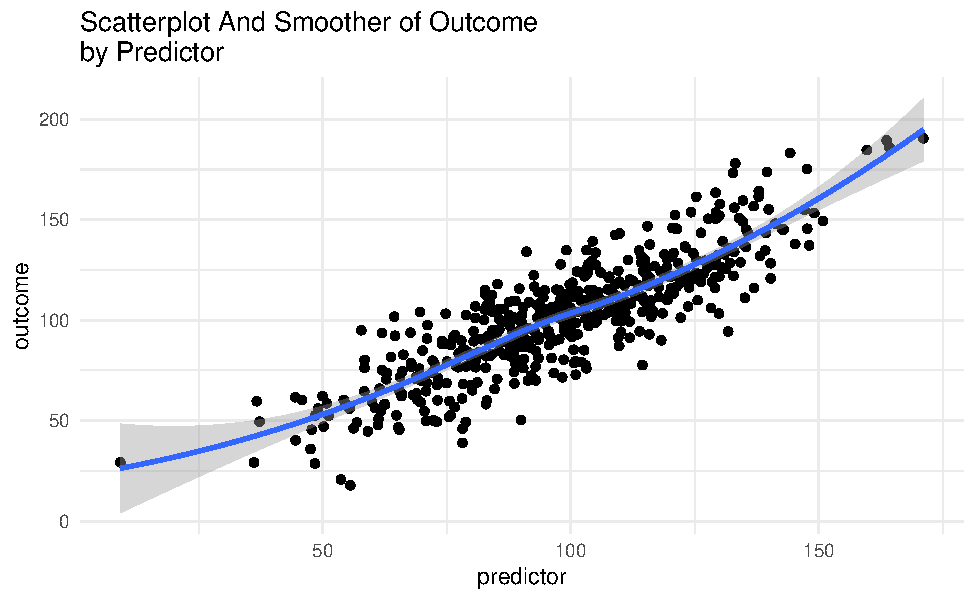
\includegraphics{introduction-to-ggplot2_files/figure-latex/unnamed-chunk-25-1.pdf}

\hypertarget{themes-requiring-ggthemes}{%
\paragraph{\texorpdfstring{Themes requiring
\texttt{ggthemes()}}{Themes requiring ggthemes()}}\label{themes-requiring-ggthemes}}

\begin{quote}
The themes below make use of \texttt{library(ggthemes)} which you will
need to install.
\end{quote}

\hypertarget{theme}{%
\subparagraph{``538'' Theme}\label{theme}}

\begin{Shaded}
\begin{Highlighting}[]
\NormalTok{p4 }\OperatorTok{+}\StringTok{ }
\StringTok{  }\KeywordTok{geom_point}\NormalTok{() }\OperatorTok{+}\StringTok{ }\CommentTok{# point geom}
\StringTok{  }\KeywordTok{geom_smooth}\NormalTok{() }\OperatorTok{+}\StringTok{ }\CommentTok{# add smooth geom}
\StringTok{  }\KeywordTok{labs}\NormalTok{(}\DataTypeTok{title =}\StringTok{"Scatterplot And Smoother of Outcome }\CharTok{\textbackslash{}n}\StringTok{by Predictor"}\NormalTok{) }\OperatorTok{+}\StringTok{ }\CommentTok{# add title}
\StringTok{  }\KeywordTok{theme_fivethirtyeight}\NormalTok{() }\OperatorTok{+}\StringTok{ }\CommentTok{# "538"-like theme}
\StringTok{  }\KeywordTok{scale_color_fivethirtyeight}\NormalTok{() }\CommentTok{# "538"-like colors}
\end{Highlighting}
\end{Shaded}

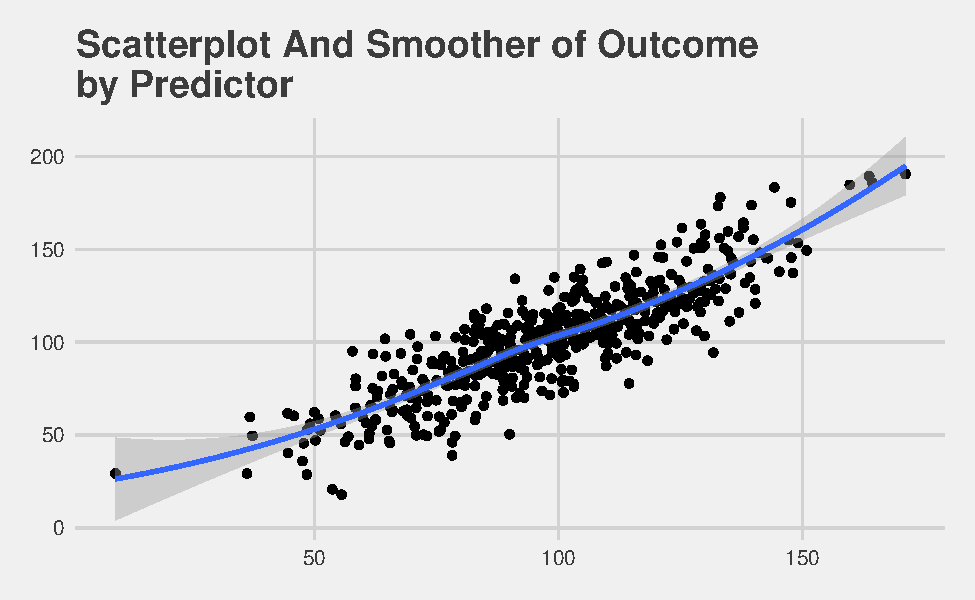
\includegraphics{introduction-to-ggplot2_files/figure-latex/unnamed-chunk-26-1.pdf}

\hypertarget{solarized-theme}{%
\subparagraph{``Solarized Theme''}\label{solarized-theme}}

\begin{Shaded}
\begin{Highlighting}[]
\NormalTok{p4 }\OperatorTok{+}\StringTok{ }
\StringTok{  }\KeywordTok{geom_point}\NormalTok{() }\OperatorTok{+}\StringTok{ }\CommentTok{# point geom}
\StringTok{  }\KeywordTok{geom_smooth}\NormalTok{() }\OperatorTok{+}\StringTok{ }\CommentTok{# add smooth geom}
\StringTok{  }\KeywordTok{labs}\NormalTok{(}\DataTypeTok{title =}\StringTok{"Scatterplot And Smoother of Outcome }\CharTok{\textbackslash{}n}\StringTok{by Predictor"}\NormalTok{) }\OperatorTok{+}\StringTok{ }\CommentTok{# add title}
\StringTok{  }\KeywordTok{theme_solarized}\NormalTok{() }\OperatorTok{+}\StringTok{ }\CommentTok{# Google Docs theme}
\StringTok{  }\KeywordTok{scale_colour_solarized}\NormalTok{() }\CommentTok{# Google Docs colors}
\end{Highlighting}
\end{Shaded}

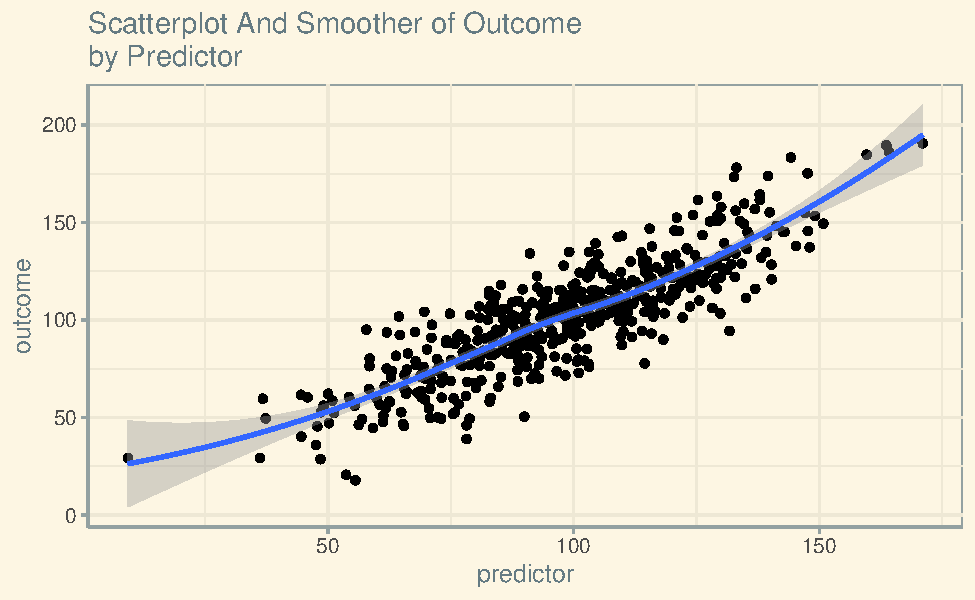
\includegraphics{introduction-to-ggplot2_files/figure-latex/unnamed-chunk-27-1.pdf}

\hypertarget{solarized-dark-theme}{%
\subparagraph{``Solarized Dark'' Theme}\label{solarized-dark-theme}}

\begin{Shaded}
\begin{Highlighting}[]
\NormalTok{p4 }\OperatorTok{+}\StringTok{ }
\StringTok{  }\KeywordTok{geom_point}\NormalTok{() }\OperatorTok{+}\StringTok{ }\CommentTok{# point geom}
\StringTok{  }\KeywordTok{geom_smooth}\NormalTok{() }\OperatorTok{+}\StringTok{ }\CommentTok{# add smooth geom}
\StringTok{  }\KeywordTok{labs}\NormalTok{(}\DataTypeTok{title =}\StringTok{"Scatterplot And Smoother of Outcome }\CharTok{\textbackslash{}n}\StringTok{by Predictor"}\NormalTok{) }\OperatorTok{+}\StringTok{ }\CommentTok{# add title}
\StringTok{  }\KeywordTok{theme_solarized}\NormalTok{(}\DataTypeTok{light =} \OtherTok{FALSE}\NormalTok{) }\OperatorTok{+}\StringTok{ }\CommentTok{# solarized dark theme}
\StringTok{  }\KeywordTok{scale_colour_solarized}\NormalTok{(}\StringTok{"blue"}\NormalTok{) }\CommentTok{# solarized dark color palette}
\end{Highlighting}
\end{Shaded}

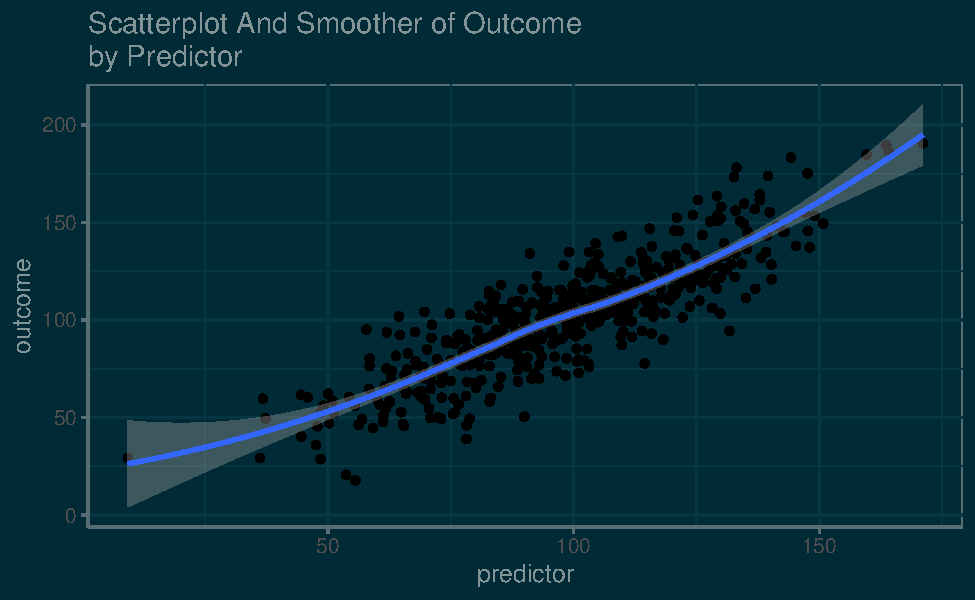
\includegraphics{introduction-to-ggplot2_files/figure-latex/unnamed-chunk-28-1.pdf}

\hypertarget{economist-theme}{%
\subparagraph{``Economist'' Theme}\label{economist-theme}}

\begin{Shaded}
\begin{Highlighting}[]
\NormalTok{p4 }\OperatorTok{+}\StringTok{ }
\StringTok{  }\KeywordTok{geom_point}\NormalTok{() }\OperatorTok{+}\StringTok{ }\CommentTok{# point geom}
\StringTok{  }\KeywordTok{geom_smooth}\NormalTok{() }\OperatorTok{+}\StringTok{ }\CommentTok{# add smooth geom}
\StringTok{  }\KeywordTok{labs}\NormalTok{(}\DataTypeTok{title =}\StringTok{"Scatterplot And Smoother of Outcome }\CharTok{\textbackslash{}n}\StringTok{by Predictor"}\NormalTok{) }\OperatorTok{+}\StringTok{ }\CommentTok{# add title}
\StringTok{  }\KeywordTok{theme_economist}\NormalTok{() }\OperatorTok{+}\StringTok{ }\CommentTok{# Economist magazine theme}
\StringTok{  }\KeywordTok{scale_colour_economist}\NormalTok{() }\CommentTok{# Economist magazine colors}
\end{Highlighting}
\end{Shaded}

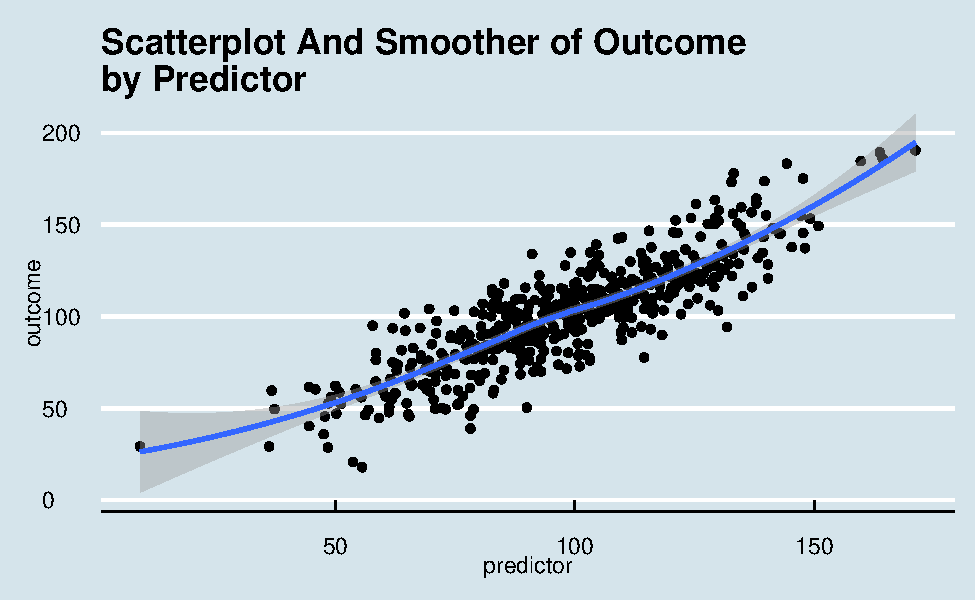
\includegraphics{introduction-to-ggplot2_files/figure-latex/unnamed-chunk-29-1.pdf}

\hypertarget{tufte-theme}{%
\subparagraph{``Tufte'' Theme}\label{tufte-theme}}

\begin{Shaded}
\begin{Highlighting}[]
\CommentTok{# same plot with theme and geom based on the work of Edward Tufte}

\NormalTok{p4 }\OperatorTok{+}\StringTok{ }
\StringTok{  }\KeywordTok{geom_point}\NormalTok{() }\OperatorTok{+}\StringTok{ }
\StringTok{  }\KeywordTok{geom_smooth}\NormalTok{(}\DataTypeTok{color =} \StringTok{"red"}\NormalTok{) }\OperatorTok{+}\StringTok{ }
\StringTok{  }\KeywordTok{theme_tufte}\NormalTok{() }\OperatorTok{+}
\StringTok{  }\KeywordTok{labs}\NormalTok{(}\DataTypeTok{title =}\StringTok{"Scatterplot And Smoother of Outcome }\CharTok{\textbackslash{}n}\StringTok{by Predictor"}\NormalTok{)}
\end{Highlighting}
\end{Shaded}

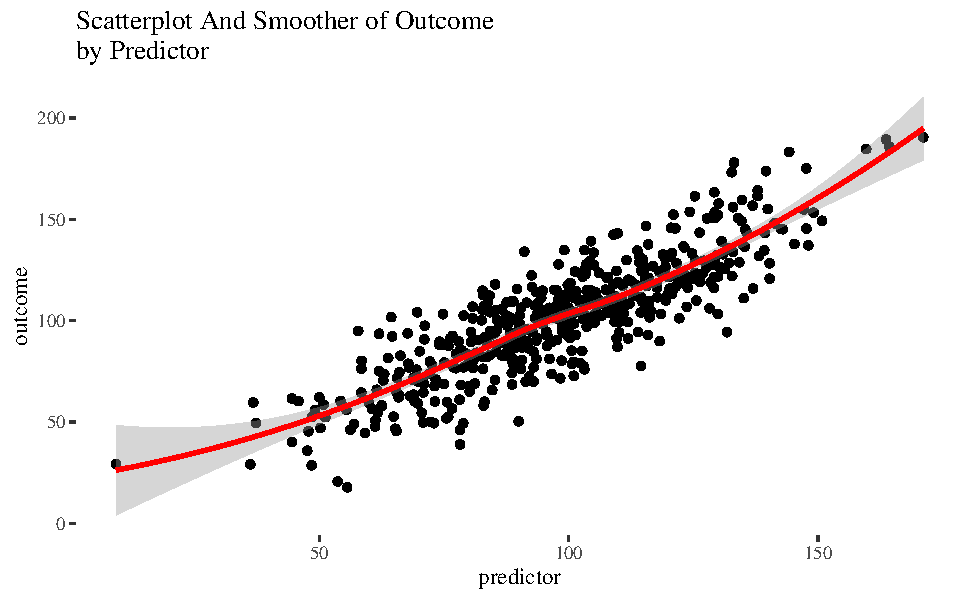
\includegraphics{introduction-to-ggplot2_files/figure-latex/unnamed-chunk-30-1.pdf}

\hypertarget{google-docs-theme}{%
\subparagraph{``Google Docs Theme''}\label{google-docs-theme}}

\begin{Shaded}
\begin{Highlighting}[]
\NormalTok{p4 }\OperatorTok{+}\StringTok{ }
\StringTok{  }\KeywordTok{geom_point}\NormalTok{() }\OperatorTok{+}\StringTok{ }\CommentTok{# point geom}
\StringTok{  }\KeywordTok{geom_smooth}\NormalTok{() }\OperatorTok{+}\StringTok{ }\CommentTok{# add smooth geom}
\StringTok{  }\KeywordTok{labs}\NormalTok{(}\DataTypeTok{title =}\StringTok{"Scatterplot And Smoother of Outcome }\CharTok{\textbackslash{}n}\StringTok{by Predictor"}\NormalTok{) }\OperatorTok{+}\StringTok{ }\CommentTok{# add title}
\StringTok{  }\KeywordTok{theme_gdocs}\NormalTok{() }\OperatorTok{+}\StringTok{ }\CommentTok{# Google Docs theme}
\StringTok{  }\KeywordTok{scale_colour_gdocs}\NormalTok{() }\CommentTok{# Google Docs colors}
\end{Highlighting}
\end{Shaded}

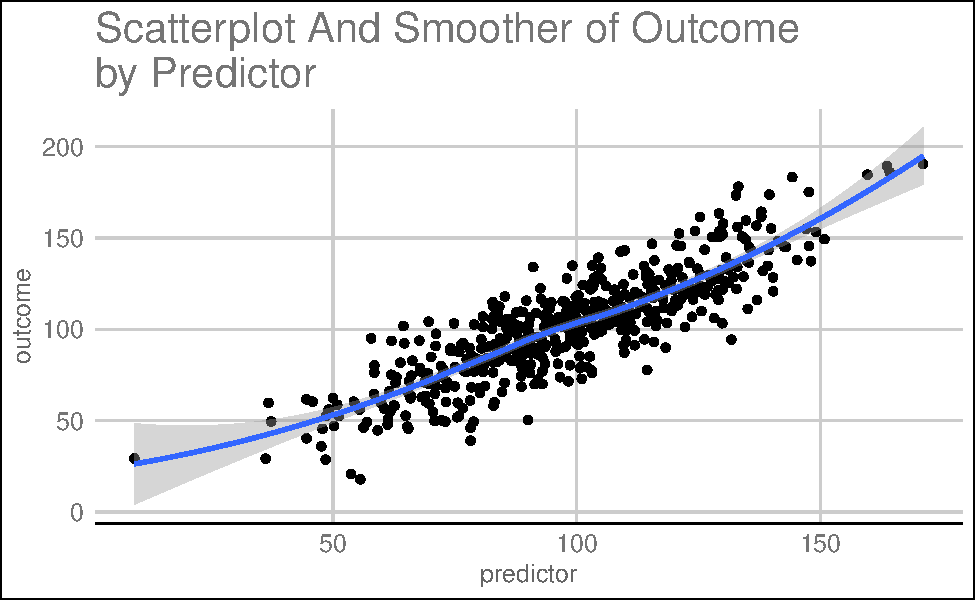
\includegraphics{introduction-to-ggplot2_files/figure-latex/unnamed-chunk-31-1.pdf}

\hypertarget{two-continous-variables-and-a-third-categorical-variable}{%
\subsection{Two Continous Variables And A Third Categorical
Variable}\label{two-continous-variables-and-a-third-categorical-variable}}

\hypertarget{modify-the-aesthetic-to-include-group.}{%
\subsubsection{\texorpdfstring{Modify the aesthetic to include
\emph{group}.}{Modify the aesthetic to include group.}}\label{modify-the-aesthetic-to-include-group.}}

\begin{Shaded}
\begin{Highlighting}[]
\NormalTok{p5 <-}\StringTok{ }\KeywordTok{ggplot}\NormalTok{(mydata, }
             \KeywordTok{aes}\NormalTok{(}\DataTypeTok{x =}\NormalTok{ predictor, }
                 \DataTypeTok{y =}\NormalTok{ outcome, }
                 \DataTypeTok{color =}\NormalTok{ group)) }\CommentTok{# aesthetic includes color by group}

\NormalTok{p5 }\OperatorTok{+}\StringTok{ }\KeywordTok{geom_point}\NormalTok{() }\OperatorTok{+}\StringTok{ }
\StringTok{  }\KeywordTok{geom_smooth}\NormalTok{() }\OperatorTok{+}\StringTok{ }
\StringTok{  }\KeywordTok{theme_economist}\NormalTok{() }\OperatorTok{+}
\StringTok{  }\KeywordTok{scale_color_economist}\NormalTok{() }\OperatorTok{+}
\StringTok{  }\KeywordTok{labs}\NormalTok{(}\DataTypeTok{title =}\StringTok{"Scatterplot And Smoother of Outcome }\CharTok{\textbackslash{}n}\StringTok{by Predictor"}\NormalTok{)}
\end{Highlighting}
\end{Shaded}

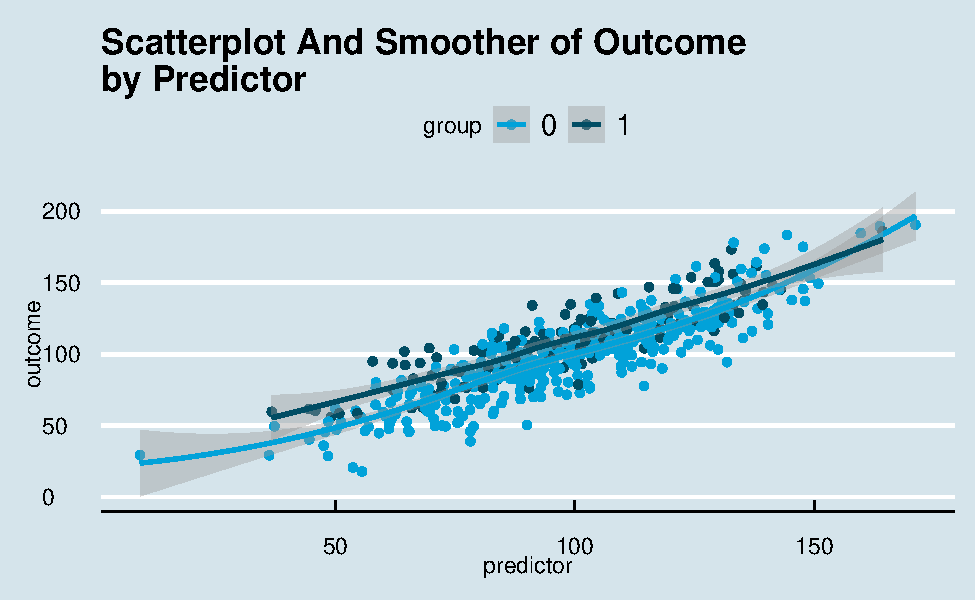
\includegraphics{introduction-to-ggplot2_files/figure-latex/unnamed-chunk-32-1.pdf}

\hypertarget{add-facets-or-small-multiples-by-group}{%
\subsubsection{Add facets or ``small multiples'' by
group}\label{add-facets-or-small-multiples-by-group}}

\begin{Shaded}
\begin{Highlighting}[]
\NormalTok{p5 }\OperatorTok{+}\StringTok{ }
\StringTok{  }\KeywordTok{geom_point}\NormalTok{() }\OperatorTok{+}\StringTok{ }
\StringTok{  }\KeywordTok{geom_smooth}\NormalTok{() }\OperatorTok{+}\StringTok{ }
\StringTok{  }\KeywordTok{facet_wrap}\NormalTok{(}\OperatorTok{~}\NormalTok{group) }\OperatorTok{+}\StringTok{ }\CommentTok{# facets or "small multiples" by group}
\StringTok{  }\KeywordTok{theme_economist}\NormalTok{() }\OperatorTok{+}
\StringTok{  }\KeywordTok{scale_color_economist}\NormalTok{() }\OperatorTok{+}
\StringTok{  }\KeywordTok{labs}\NormalTok{(}\DataTypeTok{title =}\StringTok{"Scatterplot And Smoother of Outcome }\CharTok{\textbackslash{}n}\StringTok{by Predictor"}\NormalTok{)}
\end{Highlighting}
\end{Shaded}

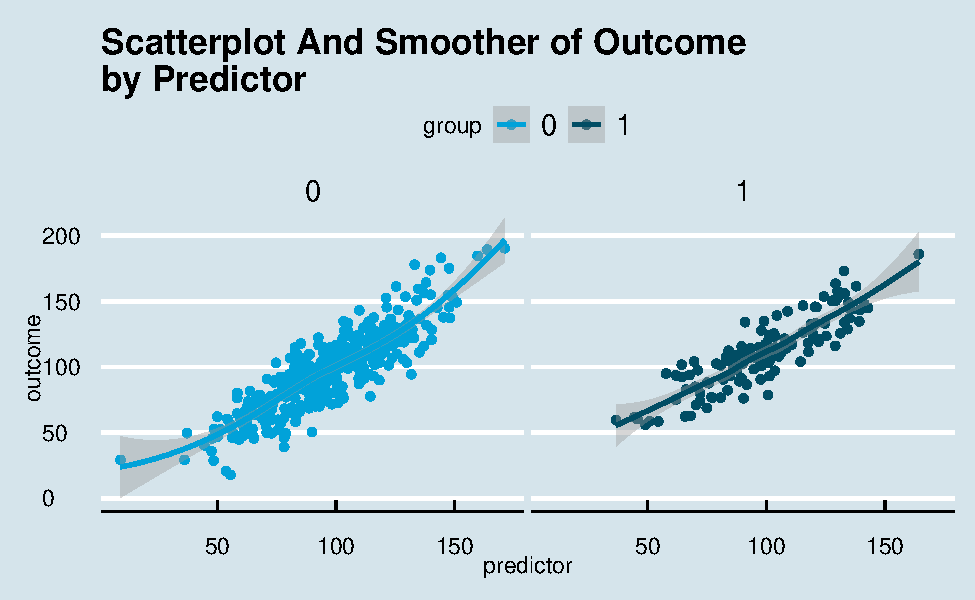
\includegraphics{introduction-to-ggplot2_files/figure-latex/unnamed-chunk-33-1.pdf}

\hypertarget{there-is-a-lot-more-that-can-be-done-with-ggplot2}{%
\section{There Is A Lot More That Can Be Done With
ggplot2}\label{there-is-a-lot-more-that-can-be-done-with-ggplot2}}

More information can be found at
\href{https://ggplot2.tidyverse.org/}{ggplot2}.

More ggplot2 examples can be found
\href{https://agrogan1.github.io/dataviz/how-to-choose-a-chart/how-to-choose-a-chart-v3.html}{here}.

\begin{center}\rule{0.5\linewidth}{\linethickness}\end{center}

Graphics made with the \href{https://ggplot2.tidyverse.org/}{ggplot2}
graphing library created by Hadley Wickham.

Available online at \url{https://www.umich.edu/~agrogan}

\emph{Quick Introduction to ggplot2} by Andrew Grogan-Kaylor is licensed
under a \href{http://creativecommons.org/licenses/by-sa/4.0/}{Creative
Commons Attribution-ShareAlike 4.0 International License}.

Last updated: \texttt{March\ 20\ 2020} at \texttt{19:38}

\end{document}
